\documentclass[
11pt, % The default document font size, options: 10pt, 11pt, 12pt
%codirector, % Uncomment to add a codirector to the title page
]{charter} 




% El títulos de la memoria, se usa en la carátula y se puede usar el cualquier lugar del documento con el comando \ttitle
\titulo{Desarrollo de aplicación para empleados SER\&PRO Services \& Products S.A. con notificación push} 

% Nombre del posgrado, se usa en la carátula y se puede usar el cualquier lugar del documento con el comando \degreename
%\posgrado{Carrera de Especialización en Sistemas Embebidos} 
\posgrado{Carrera de Especialización en Internet de las Cosas} 
%\posgrado{Carrera de Especialización en Intelegencia Artificial}
%\posgrado{Maestría en Sistemas Embebidos} 
%\posgrado{Maestría en Internet de las cosas}

% Tu nombre, se puede usar el cualquier lugar del documento con el comando \authorname
\autor{Ing. 	Fabián Alejandro Banderas Benítez} 

% El nombre del director y co-director, se puede usar el cualquier lugar del documento con el comando \supname y \cosupname y \pertesupname y \pertecosupname
\director{Mg. Ing. Yoel Yamil López}
\pertenenciaDirector{FIUBA} 
% FIXME:NO IMPLEMENTADO EL CODIRECTOR ni su pertenencia
%\codirector{Codirector a definir} % para que aparezca en la portada se debe descomentar la opción codirector en el documentclass
\pertenenciaCoDirector{FIUBA}

% Nombre del cliente, quien va a aprobar los resultados del proyecto, se puede usar con el comando \clientename y \empclientename
\cliente{Ing. Ligia Geomar Delli Valladares}
\empresaCliente{SER\&PRO Services \& Products S.A.}

% Nombre y pertenencia de los jurados, se pueden usar el cualquier lugar del documento con el comando \jurunoname, \jurdosname y \jurtresname y \perteunoname, \pertedosname y \pertetresname.
\juradoUno{Jurado a definir (1)}
\pertenenciaJurUno{FIUBA (1)} 
\juradoDos{Jurado a definir (2)}
\pertenenciaJurDos{FIUBA (2)}
\juradoTres{Jurado a definir (3)}
\pertenenciaJurTres{FIUBA (3)}
 
\fechaINICIO{21 de octubre de 2022}		%Fecha de inicio de la cursada de GdP \fechaInicioName
\fechaFINALPlan{8 de diciembre de 2022} 	%Fecha de final de cursada de GdP
\fechaFINALTrabajo{8 de diciembre de 2022}	%Fecha de defensa pública del trabajo final





\begin{document}

\maketitle
\thispagestyle{empty}
\pagebreak


\thispagestyle{empty}
{\setlength{\parskip}{0pt}
\tableofcontents{}
}
\pagebreak


\section*{Registros de cambios}
\label{sec:registro}


\begin{table}[ht]
\label{tab:registro}
\centering
\begin{tabularx}{\linewidth}{@{}|c|X|c|@{}}
\hline
\rowcolor[HTML]{C0C0C0} 
Revisión & \multicolumn{1}{c|}{\cellcolor[HTML]{C0C0C0}Detalles de los cambios realizados} & Fecha      \\ \hline
0      & Creación del documento                                 &\fechaInicioName \\ \hline
1      & Se completa hasta el punto 5 inclusive                 & 3 de noviembre de 2022 \\ \hline
2      & Se completa hasta el punto 8 inclusive                 & 10 de noviembre de 2022 \\ \hline
3      & Se completa hasta el punto 12 inclusive                 & 20 de noviembre de 2022 \\ \hline
4      & Se completa hasta el punto 17 inclusive                 & 23 de noviembre de 2022 \\ \hline
%		  Se puede agregar algo más \newline
%		  En distintas líneas \newline
%		  Así                                                    & dd/mm/aaaa \\ \hline
%3      & Se completa hasta el punto 11 inclusive                & dd/mm/aaaa \\ \hline
%4      & Se completa el plan	                                 & dd/mm/aaaa \\ \hline
\end{tabularx}
\end{table}

\pagebreak



\section*{Acta de constitución del proyecto}
\label{sec:acta}

\begin{flushright}
Guayaquil, \fechaInicioName

\end{flushright}

\vspace{2cm}

Por medio de la presente se acuerda con el \authorname\hspace{1px} que su Trabajo Final de la \degreename\hspace{1px} se titulará ``\ttitle'', consistirá esencialmente en {la implementación de un prototipo de un sistema de control de empleados}, y tendrá un presupuesto preliminar estimado de {600} hs de trabajo y {\$3764}, con fecha de inicio \fechaInicioName\hspace{1px} y fecha de presentación pública \fechaFinalName.

Se adjunta a esta acta la planificación inicial.

\vfill

% Esta parte se construye sola con la información que hayan cargado en el preámbulo del documento y no debe modificarla
\begin{table}[ht]
\centering
\begin{tabular}{ccc}
\begin{tabular}[c]{@{}c@{}}Dr. Ing. Ariel Lutenberg \\ Director posgrado FIUBA\end{tabular} & \hspace{2cm} & \begin{tabular}[c]{@{}c@{}}Ing. \clientename \\ \empclientename \end{tabular} \vspace{2.5cm} \\ 
\multicolumn{3}{c}{\begin{tabular}[c]{@{}c@{}} \supname \\ Director del Trabajo Final\end{tabular}} \vspace{2.5cm} \\
%\begin{tabular}[c]{@{}c@{}}\jurunoname \\ Jurado del Trabajo Final\end{tabular}     &  & \begin{tabular}[c]{@{}c@{}}\jurdosname\\ Jurado del Trabajo Final\end{tabular}  \vspace{2.5cm}  \\
%\multicolumn{3}{c}{\begin{tabular}[c]{@{}c@{}} \jurtresname\\ Jurado del Trabajo Final\end{tabular}} \vspace{.5cm}                                                                     
\end{tabular}
\end{table}




\section{1. Descripción técnica-conceptual del proyecto a realizar}
\label{sec:descripcion}


\begin{consigna}{black} % El bloque "consigna" se usa para poner texto en rojo y dar una pequeña ayuda sobre cómo completar la sección

Debido a la incursión de medios Smartphone, dispositivos electrónicos que se conectan a través de internet, es necesario dar una solución más sencilla para reportes de registro de entrada y salida del personal que labora en el interior de la empresa. ``En la Figura \ref{fig:diagBloques} se presenta el diagrama en bloques del sistema. Se observa que desde el dispositivo biométrico se hace el registro, este se procesa, valida, asigna de forma interna para luego extraer  enviar la notificación respectiva a quien corresponda.

A falta de un registro de entrada y salida con notificaciones para crear una mejor distribución de tiempos entre empleados se presenta la propuesta que consta de:

\begin{itemize}
	\item Supervisor
	\item Empleados
	\item Destinatarios para recibir notificación
	\item Registros
\end{itemize}

Los dispositivos a través los cuales se generan los registros, se conectarán para enviar los datos e intercambiarlos con los diferentes dispositivos. Los requerimientos mínimos se muestran a continuación:

\begin{itemize}
	\item La aplicación permite la autenticación de los miembros registrados.
	\item El empleado hará el registro de ingreso.
	\item El supervisor y personal recibirá la notificación push de ingreso.
	\item El cambio de estado y el tiempo de estancia empezará.
	\item El empleado hará el registro de salida.
	\item El supervisor y personal recibirá la notificación push de salida.
	\item Las métricas de cada uno de los empleados deben ser visuales a través de grafos.
\end{itemize}

%\vspace{25px}

\begin{figure}[htpb]
\centering 
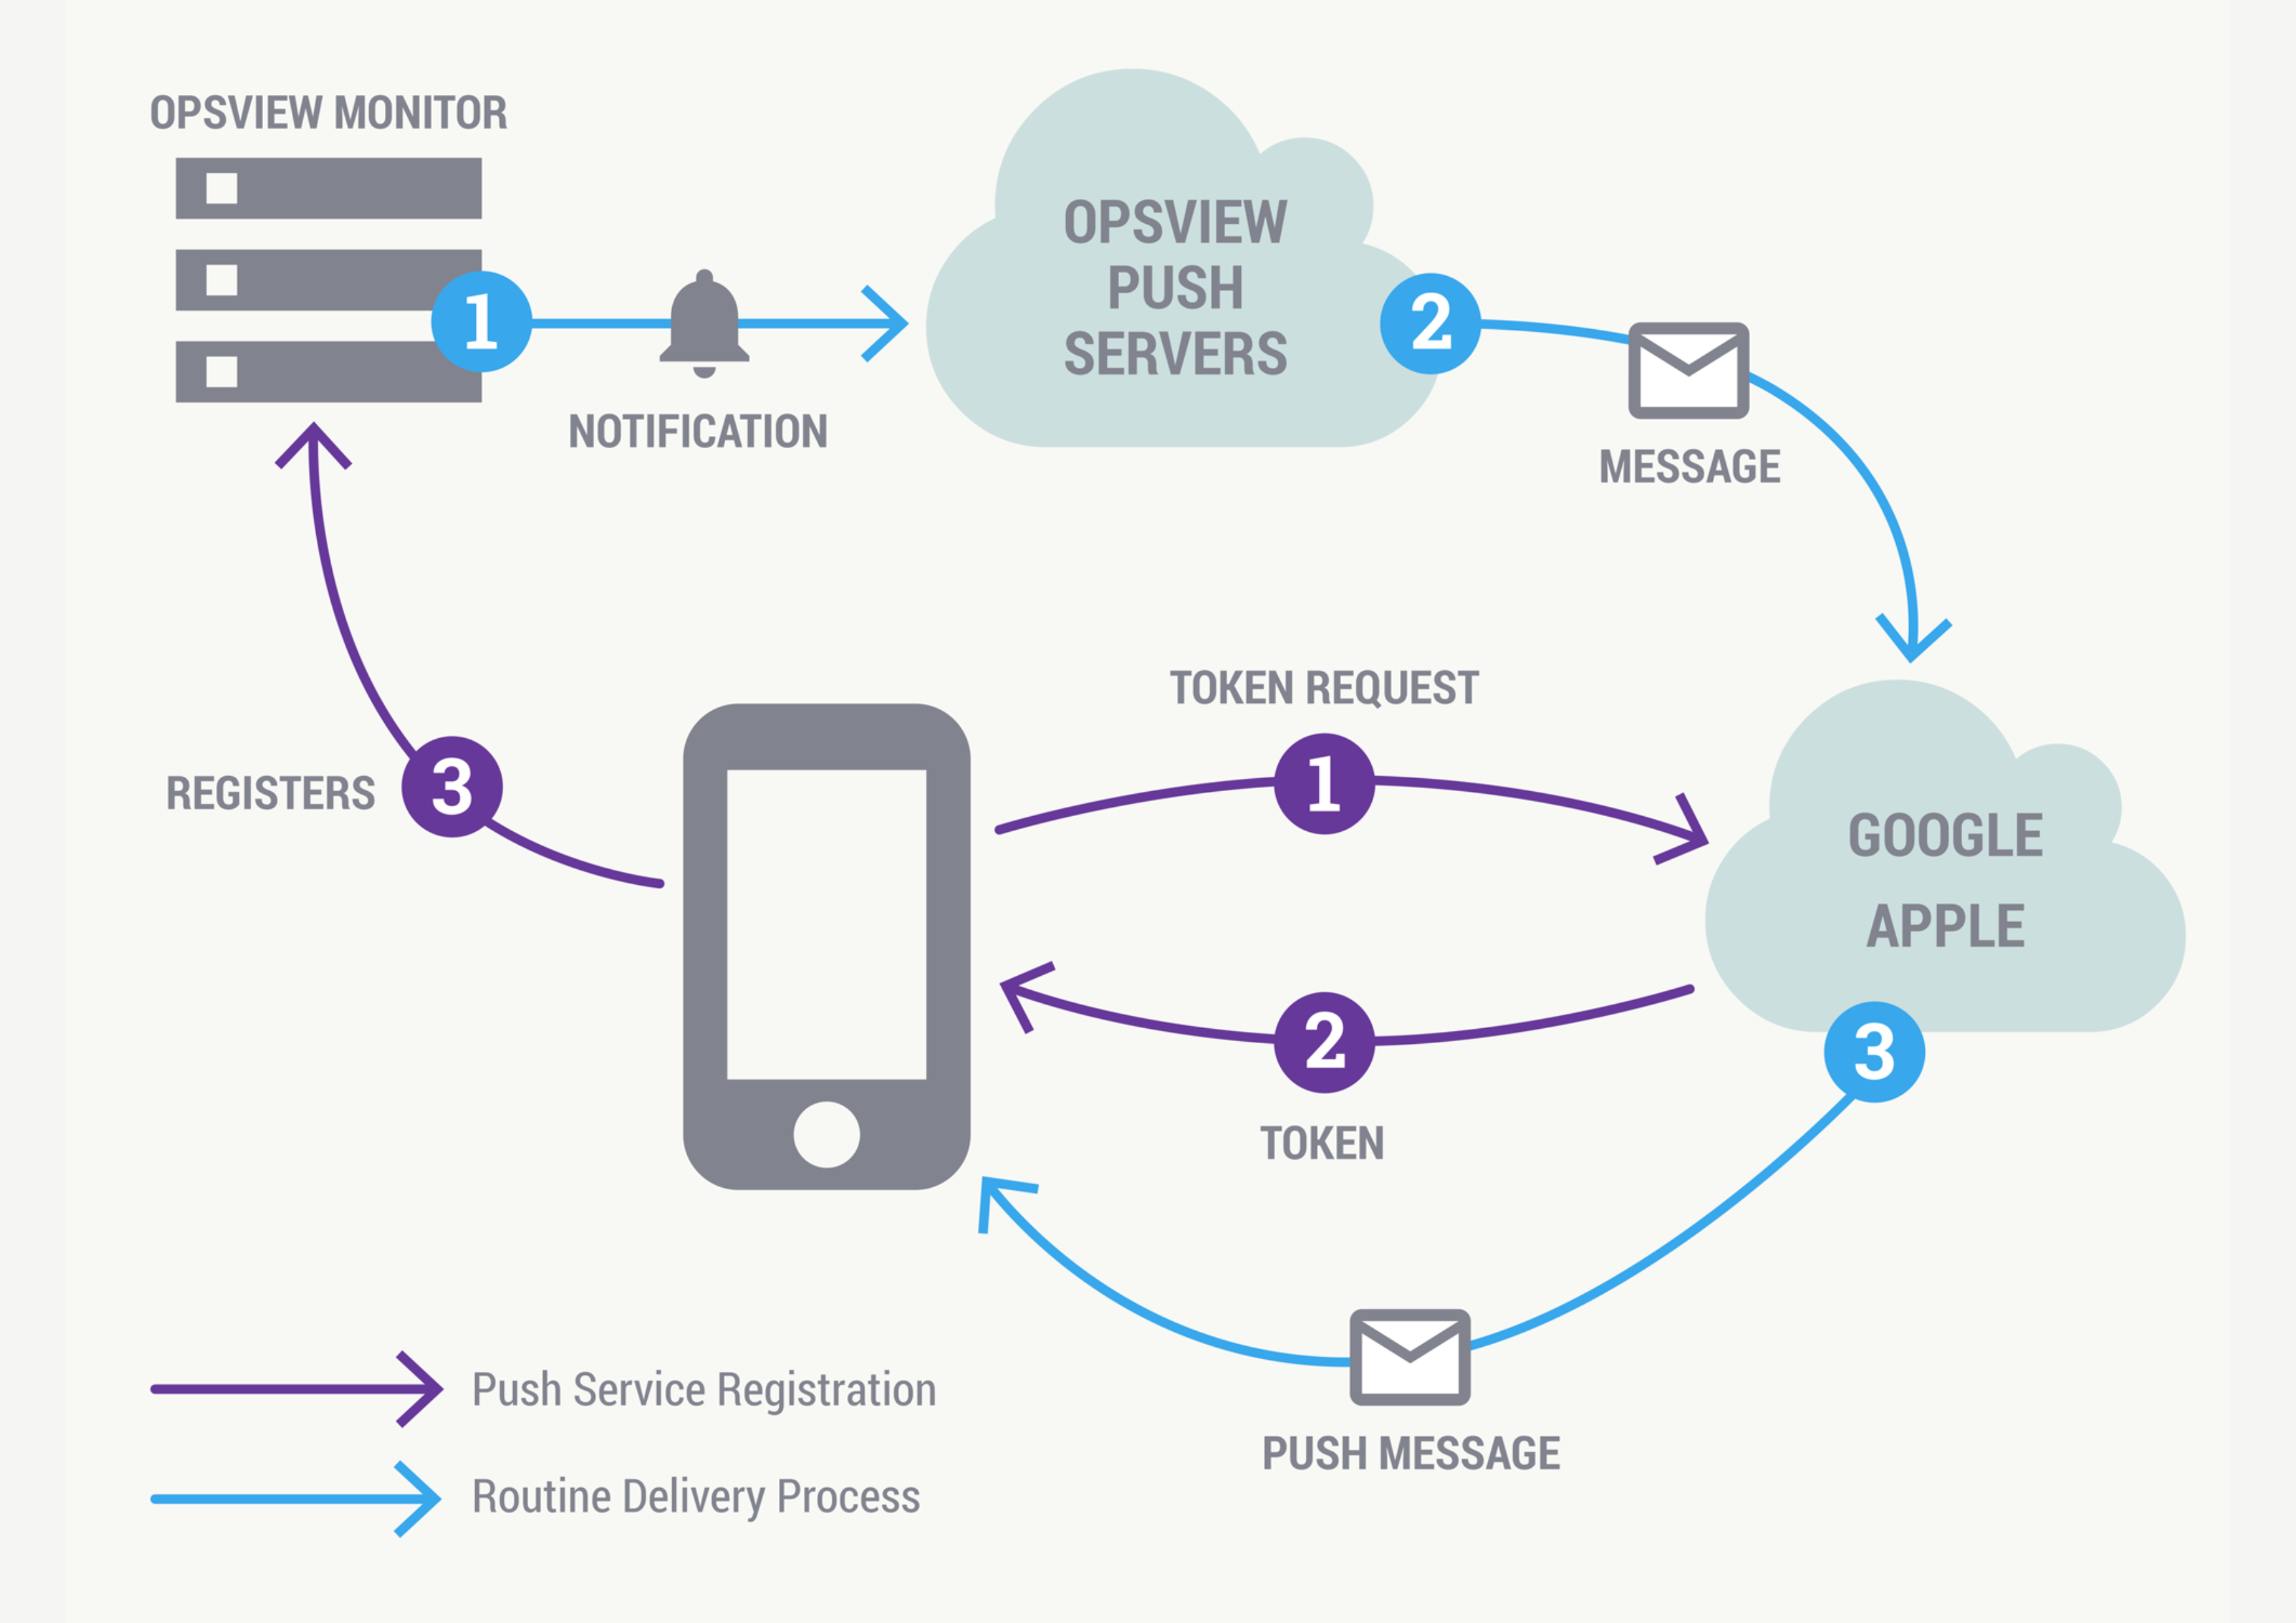
\includegraphics[width=0.85\textwidth]{./Figuras/diagBloques.png}
\caption{Diagrama en bloques del sistema.}
\label{fig:diagBloques}
\end{figure}

\vspace{25px}

\end{consigna}


\section{2. Identificación y análisis de los interesados}
\label{sec:interesados}



\begin{table}[ht]
%\caption{Identificación de los interesados}
%\label{tab:interesados}
\begin{tabularx}{\linewidth}{@{}|l|X|X|l|@{}}
\hline
\rowcolor[HTML]{C0C0C0} 
Rol           & Nombre y Apellido & Organización 	& Puesto 	\\ \hline
Auspiciante   & \clientename      &\empclientename	& Gerente  	\\ \hline
Cliente       & \clientename      &\empclientename	& Gerente  	\\ \hline
Impulsor      & Ing. Flavio Bolívar Vinueza Barzola \newline
Ing. Dennys Alejandro Montero Huilca &\empclientename	& Supervisor\\ \hline
Responsable   & \authorname       & FIUBA        	& Alumno 	\\ \hline
Colaboradores & Sr. Maike Rafael Alvarado Melendez \newline
Sr. Denny Alberto Cuzme Morales &\empclientename 	& Producción\\ \hline
Orientador    & \supname	      & \pertesupname 	& Director Trabajo final \\ \hline
Equipo        & Ing. Flavio Bolívar Vinueza Barzola \newline
				Ing. Dennys Alejandro Montero Huilca \newline 
				Sr. Maike Rafael Alvarado Melendez \newline
				Sr. Denny Alberto Cuzme Morales & \empclientename	& Empleados \\ \hline
Opositores    & Sra. Grace Ivonne Maridueña Carlier & Serintu S.A. & Gerente General \\ \hline
Usuario final & Ing. Gabriela Salvador & \empclientename	&    RRHH   	\\ \hline
\end{tabularx}
\end{table}



\section{3. Propósito del proyecto}
\label{sec:proposito}



\begin{consigna}{black}
 ``El propósito de este proyecto es mostrar mensajes informativos desde la aplicación para los usuarios con llamadas a la acción personalizadas con el fin de comunicar al usuario final.''.
 
\end{consigna}

\section{4. Alcance del proyecto}
\label{sec:alcance}




El presente proyecto contempla la notificación de los registros, entrada,
tiempo, duración y salida del mes de cada empleado en la empresa \empclientename, con el uso de una herramienta digital. Para el desarrollo del proyecto se hace uso de la metodología SCRUM.

El presente proyecto no incluye el mantenimiento de la infraestructura digital y física del
aplicativo.




\section{5. Supuestos del proyecto}
\label{sec:supuestos}



Para el desarrollo del presente proyecto se supone que: 

\begin{itemize}
	\item La disponibilidad del cliente Ing. \clientename, impulsores o colaboradores encargados para la guía en el avance del proyecto. 
	\item Los recursos actuales pueden ser modernizados por necesidad propia de la empresa.
	\item Cambios o implementación de leyes para regulación nacional para el uso de los equipos.
	\item Cambios del personal de la empresa.
	\item Cambios en directrices de la empresa.
	\item Prioridades de la empresa por eventos inesperados.
	\item Fenómenos naturales.
	\item Daño del lector biométrico LX50 ZK.
	\item Corte de energía.
\end{itemize}



\section{6. Requerimientos}
\label{sec:requerimientos}


\begin{enumerate}
	\item Requerimientos funcionales
		\begin{enumerate}
			\item El empleado se registra en el sistema.
			\item El sistema debe autenticar solo a los empleados de planta de la empresa registrados.
			\item El supervisor y empleado reciben una notificación push de ingreso al sistema.
			\item El supervisor y usuario pueden ver el tiempo de estancia que tuvo un empleado en la empresa en un determinado tiempo.
			\item El supervisor y empleado reciben una notificación push del reporte ingresos a la empresa.
			\item El supervisor y usuario reciben una notificación push del reporte de salida de la empresa.
			\item El supervisor tiene acceso al reporte de tiempo promedio promedio del empleado en la empresa en un rango de fechas. 
			\item Cada empleado tiene un registro de entradas, salidas con tiempos de estancia que se pueden ver a través de grafos.
			\item El empleado puede ver el tiempo de estancia total  que tuvo en un rango de fechas desde realizó el registro de usuario en el sistema.
		\end{enumerate}
	\item Requerimientos de documentación
		\begin{enumerate}
			\item Manual de usuario.
			\item Planilla de casos de uso.
		\end{enumerate}
	\item Requerimiento de testing
		\begin{enumerate}
			\item Validación de datos para el registro del sistema.
			\item Notificación push para el empleado.
			\item Notificación push para el supervisor.
		\end{enumerate}
	\item Requerimientos de la interfaz.
			\begin{enumerate}
			\item Debe contar con los distintivos de la empresa y colores de marca.
			\item Usar técnica de ingeniería de software para el diseño de la interfaz de usuario.
		\end{enumerate}
	\item Requerimientos interoperabilidad.
			\begin{enumerate}
			\item El usuario puede ingresar a su perfil de empleado con credenciales únicas.
			\item El supervisor puede visualizar métricas de todos los empleados.
			\item Realizar la evaluación de usabilidad de la aplicación mediante el uso de la Norma ISO/IEC 25010.
		\end{enumerate}
\end{enumerate}



\section{7. Historias de usuarios (\textit{Product backlog})}
\label{sec:backlog}


Para realizar la estimación de puntos estimados del proyecto se emplea la famosa serie Fibonacci, que se describe en la siguiente tabla.

\begin{table}[H]
%\label{tab:puntos estimados - horas de trabajo}
\centering
 \begin{tabular}{|c|p{14cm}|} 
\hline
\rowcolor[HTML]{C0C0C0} 
\multicolumn {2}{|c|}{\textbf{Fibonacci Práctico}}  	\\ \hline
0  & No se requiere esfuerzo, o se requiere algo de esfuerzo, pero no se entrega ningún valor comercial, por lo que no se acumulan Puntos por hacer el trabajo. Un ejemplo es un cambio de comportamiento deseado derivado de la Retrospectiva de Scrum.¨ \\ \hline
1  & Extra Pequeño. Los desarrolladores sienten que entienden la mayoría de los requisitos y lo consideran relativamente fácil, probablemente el elemento más pequeño del Sprint y probablemente completado en un día. \\ \hline
2  & Pequeña. Se requiere un poco de pensamiento, esfuerzo o resolución de problemas, pero los desarrolladores han hecho esto mucho, por lo que confían en los requisitos. O bien, suena muy pequeño, pero quieren cubrir su apuesta un poco.  \\ \hline
3  & Promedio. Los desarrolladores han hecho esto mucho; ellos saben lo que hay que hacer. Puede haber algunos pasos adicionales, pero eso es todo. Es dudoso que necesiten investigar algo. \\ \hline
5  & Largo. Este es un trabajo complejo, o los desarrolladores no lo hacen muy a menudo. La mayoría de los desarrolladores necesitarán la ayuda de otra persona del equipo. Este es probablemente uno de los elementos más grandes que se pueden completar dentro de un Sprint. \\ \hline
8  & Extra grande. Esto llevará algo de tiempo e investigación y probablemente más de un desarrollador lo complete en dos semanas. Además, los desarrolladores deben hacer varias suposiciones que aumentan el riesgo y podrían afectar su realización. \\ \hline
13  & ¡Advertencia!  Este es un trabajo complejo con muchas incógnitas y requiere múltiples suposiciones para dimensionar. Es demasiado para completar en un Sprint. En su lugar, divida esto en varios elementos que se pueden completar de forma independiente. \\ \hline
21  & ¡Peligro!  Un ''21''o''34'' refleja demasiada complejidad para realizar dentro de un Sprint. Habrá que afinar más. El tamaño grande también indica más riesgos, suposiciones y dependencias involucradas para completar este elemento.\\ \hline
?   & ¡Peligro! Como desarrollador, no queremos hacer este trabajo de la forma en que está escrito actualmente. Es muy complejo y no se puede completar en el tiempo de una iteración o Sprint. Quizás los requisitos son tan confusos que está plagado de peligros.\\ \hline
%\end{tabularx}
\end{tabular}
\end{table}

%Historia de usuario Requerimientos funcionales
% 1	\item El empleado se registra en el sistema.
% 2	\item El sistema debe autenticar solo a los empleados de planta de la empresa registrados.
% 3	\item El supervisor y empleado reciben una notificación push de ingreso al sistema.
% 4 \item El supervisor y usuario pueden ver el tiempo de estancia que tuvo un empleado en la empresa en un determinado tiempo.
% 5	\item El supervisor y empleado reciben una notificación push del reporte ingresos a la empresa.
% 6	\item El supervisor y usuario reciben una notificación push del reporte de salida de la empresa.
% 7	\item El supervisor tiene acceso al reporte de tiempo promedio promedio del empleado en la empresa en un rango de fechas. 
% 8	\item Cada empleado tiene un registro de entradas, salidas con tiempos de estancia que se pueden ver a través de grafos.
% 9	\item El empleado puede ver el tiempo de estancia total  que tuvo en un rango de fechas desde realizó el registro de usuario en el sistema.


%\label{Historia de usuario 1}
\begin{table}[H]
 \begin{tabular}{|l|l|}
\hline
\rowcolor[HTML]{C0C0C0} 
\multicolumn {2}{|r|}{\textbf{Historia de Usuario}}  	\\ \hline
\textbf{Número:} 1 & \textbf{Usuario:} \clientename \\ \hline
\multicolumn {2}{|p{14cm}|}{ \textbf{Nombre historia:} El empleado se registra en el sistema.}\\ \hline
\textbf{Prioridad del negocio:} ALTA & \textbf{Riesgo en desarrollo:} BAJA \\ \hline
\textbf{Puntos estimados:} 8 & \textbf{Iteración asignada:} 1 \\ \hline
\multicolumn {2}{|p{14cm}|}{ \textbf{Programador Responsable:} \authorname}\\ \hline
\multicolumn {2}{|p{14cm}|}{ \textbf{Descripción:} \newline
Como cliente quiero que cada empleado se registre en el sistema con los datos de empresa que tiene asignado.}\\ \hline
\multicolumn {2}{|p{14cm}|}{ \textbf{Validación:} \newline
Solo si el código de empleado de planta coincide con el código de la base de datos de empleados de planta permite registrarse en el aplicativo.}\\ \hline
%\end{tabularx}
\end{tabular}
\end{table}

%\label{Historia de usuario 2}
\begin{table}[H]
 \begin{tabular}{|l|l|}
\hline
\rowcolor[HTML]{C0C0C0} 
\multicolumn {2}{|r|}{\textbf{Historia de Usuario}}  	\\ \hline
\textbf{Número:} 2 & \textbf{Usuario:} \clientename \\ \hline
\multicolumn {2}{|p{14cm}|}{ \textbf{Nombre historia:} El sistema debe autenticar solo a los empleados de planta de la empresa registrados.}\\ \hline
\textbf{Prioridad del negocio:} ALTA & \textbf{Riesgo en desarrollo:} BAJA \\ \hline
\textbf{Puntos estimados:} 8 & \textbf{Iteración asignada:} 1 \\ \hline
\multicolumn {2}{|p{14cm}|}{ \textbf{Programador Responsable:} \authorname}\\ \hline
\multicolumn {2}{|p{14cm}|}{ \textbf{Descripción:} \newline
Como cliente quiero que solo se autentifiquen los empleados de planta la empresa para no tener otras personas.}\\ \hline
\multicolumn {2}{|p{14cm}|}{ \textbf{Validación:} \newline
Solo la credencial válida de empleado de planta permite autenticarse en el aplicativo.}\\ \hline
%\end{tabularx}
\end{tabular}
\end{table}

%\label{Historia de usuario 3}
\begin{table}[H]
 \begin{tabular}{|l|l|}
\hline
\rowcolor[HTML]{C0C0C0} 
\multicolumn {2}{|r|}{\textbf{Historia de Usuario}}  	\\ \hline
\textbf{Número:} 3 & \textbf{Usuario:} \clientename \\ \hline
\multicolumn {2}{|p{14cm}|}{ \textbf{Nombre historia:} El supervisor y empleado reciben una notificación push de ingreso al sistema.}\\ \hline
\textbf{Prioridad del negocio:} MEDIA & \textbf{Riesgo en desarrollo:} BAJA \\ \hline
\textbf{Puntos estimados:} 5 & \textbf{Iteración asignada:} 2 \\ \hline
\multicolumn {2}{|p{14cm}|}{ \textbf{Programador Responsable:} \authorname}\\ \hline
\multicolumn {2}{|p{14cm}|}{ \textbf{Descripción:} \newline
Como cliente quiero que cuando ingrese el usuario en el aplicativo reciba un mensaje inmediato a través de correo electrónico de aviso.}\\ \hline
\multicolumn {2}{|p{14cm}|}{ \textbf{Validación:} \newline
Después de autentificarse el empleado en el sistema, de forma automática debe recibir una notificación de aviso en bandeja de correo electrónico.}\\ \hline
%\end{tabularx}
\end{tabular}
\end{table}

%\label{Historia de usuario 4}
\begin{table}[H]
 \begin{tabular}{|l|l|}
\hline
\rowcolor[HTML]{C0C0C0} 
\multicolumn {2}{|r|}{\textbf{Historia de Usuario}}  	\\ \hline
\textbf{Número:} 4 & \textbf{Usuario:} \clientename \\ \hline
\multicolumn {2}{|p{14cm}|}{ \textbf{Nombre historia:} El supervisor y usuario pueden ver el tiempo de estancia que tuvo un empleado en la empresa en un determinado tiempo.}\\ \hline
\textbf{Prioridad del negocio:} MEDIA & \textbf{Riesgo en desarrollo:} BAJA \\ \hline
\textbf{Puntos estimados:} 8 & \textbf{Iteración asignada:} 3 \\ \hline
\multicolumn {2}{|p{14cm}|}{ \textbf{Programador Responsable:} \authorname}\\ \hline
\multicolumn {2}{|p{14cm}|}{ \textbf{Descripción:} \newline
Como cliente quiero que cada empleado pueda ver el tiempo que estuvo o está en la empresa en una fecha específica para que vea la estancia que tuvo en una fecha determinada.}\\ \hline
\multicolumn {2}{|p{14cm}|}{ \textbf{Validación:} \newline
Cuando el empleado este en su perfil seleccione una fecha determinada y se muestre un gráfico con el tiempo que está o ha pasado en una fecha determinada.}\\ \hline
%\end{tabularx}
\end{tabular}
\end{table}

%\label{Historia de usuario 5}
\begin{table}[H]
 \begin{tabular}{|l|l|}
\hline
\rowcolor[HTML]{C0C0C0} 
\multicolumn {2}{|r|}{\textbf{Historia de Usuario}}  	\\ \hline
\textbf{Número:} 5 & \textbf{Usuario:} \clientename \\ \hline
\multicolumn {2}{|p{14cm}|}{ \textbf{Nombre historia:} El supervisor y empleado reciben una notificación push del reporte ingresos a la empresa.}\\ \hline
\textbf{Prioridad del negocio:} MEDIA & \textbf{Riesgo en desarrollo:} BAJA \\ \hline
\textbf{Puntos estimados:} 8 & \textbf{Iteración asignada:} 3 \\ \hline
\multicolumn {2}{|p{14cm}|}{ \textbf{Programador Responsable:} \authorname}\\ \hline
\multicolumn {2}{|p{14cm}|}{ \textbf{Descripción:} \newline
Como cliente quiero que cada empleado pueda ver el tiempo que estuvo o está en la empresa en una fecha específica para que vea la estancia que tuvo en una fecha determinada.}\\ \hline
\multicolumn {2}{|p{14cm}|}{ \textbf{Validación:} \newline
Cuando el empleado este en su perfil seleccione una fecha determinada y se muestre un gráfico con el tiempo que está o ha pasado en una fecha determinada.}\\ \hline
%\end{tabularx}
\end{tabular}
\end{table}

%\label{Historia de usuario 6}
\begin{table}[H]
 \begin{tabular}{|l|l|}
\hline
\rowcolor[HTML]{C0C0C0} 
\multicolumn {2}{|r|}{\textbf{Historia de Usuario}}  	\\ \hline
\textbf{Número:} 6 & \textbf{Usuario:} \clientename \\ \hline
\multicolumn {2}{|p{14cm}|}{ \textbf{Nombre historia:} El supervisor y usuario reciben una notificación push del reporte de salida de la empresa.}\\ \hline
\textbf{Prioridad del negocio:} MEDIA & \textbf{Riesgo en desarrollo:} BAJA \\ \hline
\textbf{Puntos estimados:} 8 & \textbf{Iteración asignada:} 4 \\ \hline
\multicolumn {2}{|p{14cm}|}{ \textbf{Programador Responsable:} \authorname}\\ \hline
\multicolumn {2}{|p{14cm}|}{ \textbf{Descripción:} \newline
Como cliente quiero que cada empleado pueda ver la hora a la que sale de la empresa en una fecha específica para que vea la estancia de salida y recibe una notificación push de aviso.}\\ \hline
\multicolumn {2}{|p{14cm}|}{ \textbf{Validación:} \newline
Cuando el empleado registre su salida de la empresa se tendrá el valor de salida con el cual se construye el gráfico de estancia por día.}\\ \hline
%\end{tabularx}
\end{tabular}
\end{table}


%\label{Historia de usuario 7}
\begin{table}[H]
 \begin{tabular}{|l|l|}
\hline
\rowcolor[HTML]{C0C0C0} 
\multicolumn {2}{|r|}{\textbf{Historia de Usuario}}  	\\ \hline
\textbf{Número:} 7 & \textbf{Usuario:} \clientename \\ \hline
\multicolumn {2}{|p{14cm}|}{ \textbf{Nombre historia:} El supervisor tiene acceso al reporte de tiempo promedio promedio del empleado en la empresa en un rango de fechas.}\\ \hline
\textbf{Prioridad del negocio:} ALTA & \textbf{Riesgo en desarrollo:} BAJA \\ \hline
\textbf{Puntos estimados:} 8 & \textbf{Iteración asignada:} 5 \\ \hline
\multicolumn {2}{|p{14cm}|}{ \textbf{Programador Responsable:} \authorname}\\ \hline
\multicolumn {2}{|p{14cm}|}{ \textbf{Descripción:} \newline
Como cliente quiero que el supervisor pueda visualizar el reporte de tiempo promedio de un rango de fechas para obtener métricas de cada uno de los empleados de la empresa.}\\ \hline
\multicolumn {2}{|p{14cm}|}{ \textbf{Validación:} \newline
Cuando el supervisor seleccione la fecha de inicio y la fecha de fin de rango debe visualizar a traves de grafos el reporte.}\\ \hline
%\end{tabularx}
\end{tabular}
\end{table}

%\label{Historia de usuario 8}
\begin{table}[H]
 \begin{tabular}{|l|l|}
\hline
\rowcolor[HTML]{C0C0C0} 
\multicolumn {2}{|r|}{\textbf{Historia de Usuario}}  	\\ \hline
\textbf{Número:} 8 & \textbf{Usuario:} \clientename \\ \hline
\multicolumn {2}{|p{14cm}|}{ \textbf{Nombre historia:} Cada empleado tiene un registro de entradas, salidas con tiempos de estancia que se pueden ver a través de grafos.}\\ \hline
\textbf{Prioridad del negocio:} ALTA & \textbf{Riesgo en desarrollo:} BAJA \\ \hline
\textbf{Puntos estimados:} 8 & \textbf{Iteración asignada:} 5 \\ \hline
\multicolumn {2}{|p{14cm}|}{ \textbf{Programador Responsable:} \authorname}\\ \hline
\multicolumn {2}{|p{14cm}|}{ \textbf{Descripción:} \newline
Como cliente quiero que el supervisor pueda visualizar el reporte de tiempo promedio del empleado un rango de fechas y de los empleados en promedio para obtener métricas generales de los empleados de la empresa.}\\ \hline
\multicolumn {2}{|p{14cm}|}{ \textbf{Validación:} \newline
Cuando el supervisor seleccione la fecha de inicio y la fecha de fin de rango debe visualizar a traves de grafos el reporte general de los empleados.}\\ \hline
%\end{tabularx}
\end{tabular}
\end{table}


%\label{Historia de usuario 9}
\begin{table}[H]
 \begin{tabular}{|l|l|}
\hline
\rowcolor[HTML]{C0C0C0} 
\multicolumn {2}{|r|}{\textbf{Historia de Usuario}}  	\\ \hline
\textbf{Número:} 9 & \textbf{Usuario:} \clientename \\ \hline
\multicolumn {2}{|p{14cm}|}{ \textbf{Nombre historia:} El empleado puede ver el tiempo de estancia total  que tuvo en un rango de fechas desde realizó el registro de usuario en el sistema.}\\ \hline
\textbf{Prioridad del negocio:} ALTA & \textbf{Riesgo en desarrollo:} BAJA \\ \hline
\textbf{Puntos estimados:} 8 & \textbf{Iteración asignada:} 5 \\ \hline
\multicolumn {2}{|p{14cm}|}{ \textbf{Programador Responsable:} \authorname}\\ \hline
\multicolumn {2}{|p{14cm}|}{ \textbf{Descripción:} \newline
Como cliente quiero que cada empleado pueda ver su reporte de estancia en la empresa en un rango de fechas y de los empleados para que visualice el comportamiento personal con respecto al tiempo empleado en la empresa.}\\ \hline
\multicolumn {2}{|p{14cm}|}{ \textbf{Validación:} \newline
Cuando el empleado seleccione la fecha de inicio y la fecha de fin de rango debe visualizar el a traves de gráfico de barras el reporte de tiempo por cada día en el rango de fecha seleccionada.}\\ \hline
%\end{tabularx}
\end{tabular}
\end{table}


\section{8. Entregables principales del proyecto}
\label{sec:entregables}



Los entregables del proyecto son:

\begin{itemize}
	\item Diagrama de estructura de la organización registrada.
	\item Diagrama de los valores utilizados en el lector biométrico LX50 ZK.
	\item Código fuente del aplicativo.
	\item Diagramas de uso. 
	\item Diseño de web \textit{assets}.
	\item Entrega de aplicativo.
	\item Test de evaluación del aplicativo.
	\item Manual de usuario.
	\item Informe final.
\end{itemize}



\section{9. Desglose del trabajo en tareas}
\label{sec:wbs}


\begin{enumerate}
\item Planificación del proyecto (60 hs)
	\begin{enumerate}
	\item Reuniones con cliente. (5 hs)
	\item Análisis de requerimientos del cliente. (20 hs)
	\item Elaborar documentación. (35 hs)
	\end{enumerate}
\item Estudio preliminar (100 hs)
	\begin{enumerate}
	\item Investigación de lector biométrico LX50 ZK (20 hs)
	\item Investigación de protocolo de comunicación (10 hs)
	\item Preparación de área de trabajo (10 hs)
	\item Preparación de equipos (10 hs)
	\item Instalación de software de desarrollo (10 hs)
	\item Estudio de desarrollo cloud (20 hs)
	\item Estudio progresive web app (20 hs)
	\end{enumerate}
\item Adquisición de componentes. (20 hs)
	\begin{enumerate}
	\item Cotizar costos de lectores biométricos con proveedores. (10 hs)
	\item Realizar compra. (5 hs)
	\item Informe adquisición de productos. (10 hs)
	\end{enumerate}
\item Planificación y desarrollo del aplicativo empleados SER\&PRO (280 hs)
	\begin{enumerate}
	\item Estudio del funcionamiento de las bibliotecas para conexión LX50 ZK. (10 hs)
	\item Estudio, elaboración de certificados, repositorio y credenciales privadas. (15 hs)
	\item Desarrollo de funcionalidades haciendo referencia Norma ISO/IEC 25010. (60 hs)
	\item Pruebas y depuración de errores en la conexión y transporte del dato al servidor
central. (35 hs)
	
	\item Desarrollo de las funciones de procesamiento de la variable medida tiempo. (20 hs)
	\item Desarrollo de la pagina web de configuración. (60 hs)
	\item Pruebas del aplicativo. (40 hs)
	\item Depuración del código. (40 hs)
	\end{enumerate}
\item Implementacion de la base de datos cloud. (25 hs)
\item Administrar notificaciones. (92 hs)
	\begin{enumerate}
	\item Creación de canales en Google. (5 hs)
	\item Creación de correos y usuarios de prueba. (2 hs)
	\item Gestión de reglas para envío de notificaciones. (20 hs)
	\item Gestión de reglas dashboard para mostrar estado de empleado. (25 hs)
	\item Verificación de notificaciones ingreso empleado. (10 hs)
	\item Verificación de notificaciones salida empleado. (10 hs)
	\item Pruebas online y offline de los dispositivos. (20 hs)
	\end{enumerate}
\item Verificación de funcionalidades y cumplimiento de requisitos. (30 hs)
\item Documentación (15 hs)
	\begin{enumerate}
	\item Elaboración manual de usuario. (15 hs)
	\end{enumerate}
\end{enumerate}
Cantidad total de horas: (622 hs)


\section{10. Diagrama de Activity On Node}
\label{sec:AoN}

La unidad de tiempo del diagrama AoN que se muestra en la Figura 2 está expresada en horas.

%\label{Historia de usuario 1}
\begin{table}[H]
 \begin{tabular}{|l|l|l|}
\hline
\rowcolor[HTML]{C0C0C0} 
\textbf{Descripción} & \textbf{Secuencia de tareas} & \textbf{Tiempo (horas)} \\ \hline
Camino & 1 - 2 - 3 - 4 - 5 - 6 - 7 - 8 & 622	\\ \hline

%\end{tabularx}
\end{tabular}
\end{table}


\begin{figure}[htpb]
\centering 
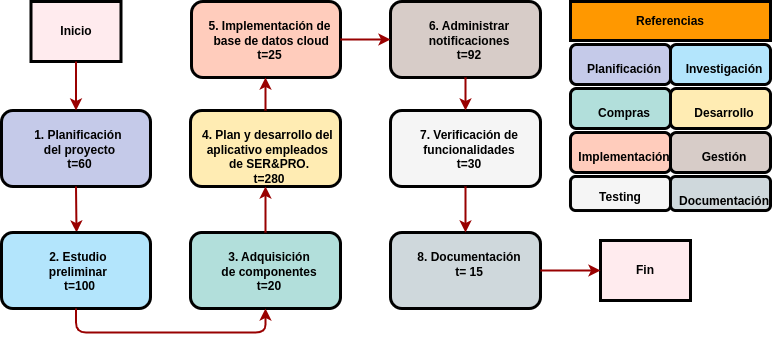
\includegraphics[width=.8\textwidth]{./Figuras/AoN.png}
\caption{Diagrama en \textit{Activity on Node}}
\label{fig:AoN}
\end{figure}




\section{11. Diagrama de Gantt}
\label{sec:gantt}


\begin{figure}[htpb]
\centering 
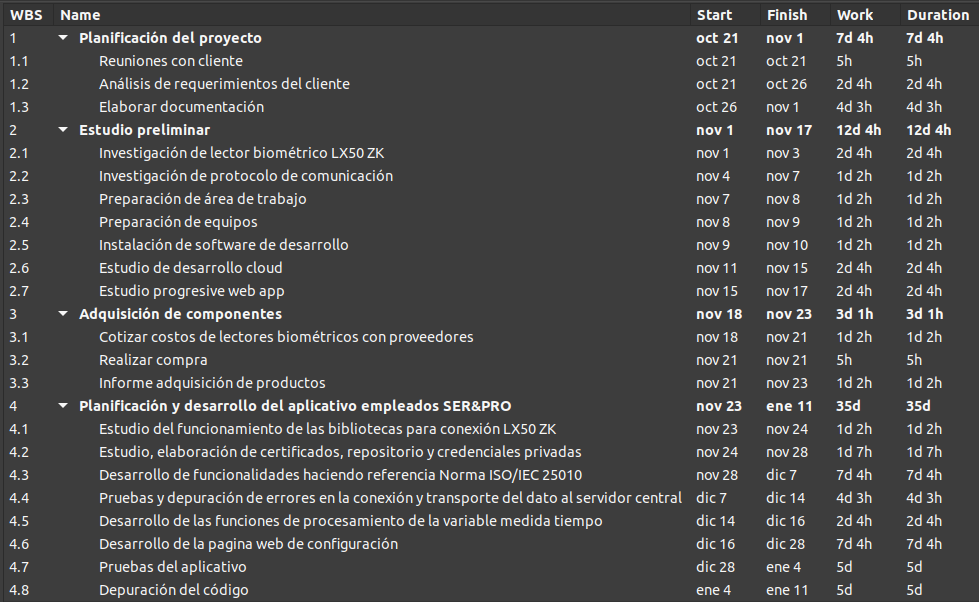
\includegraphics[width=1\textwidth]{./Figuras/GantTasks1.png}
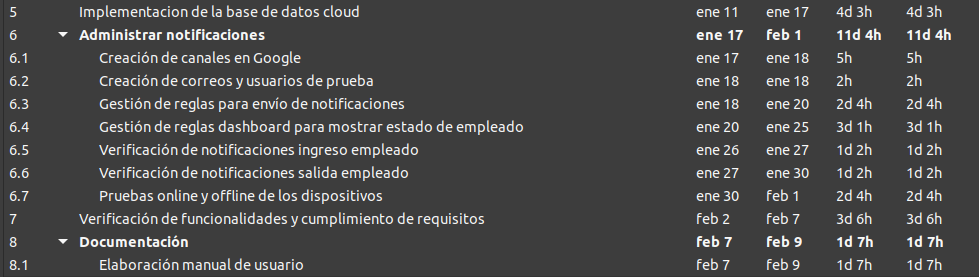
\includegraphics[width=1\textwidth]{./Figuras/GantTasks2.png}
\caption{Tabla de actividades}
\label{fig:AoN}
\end{figure}

\begin{figure}[htpb]
\centering 
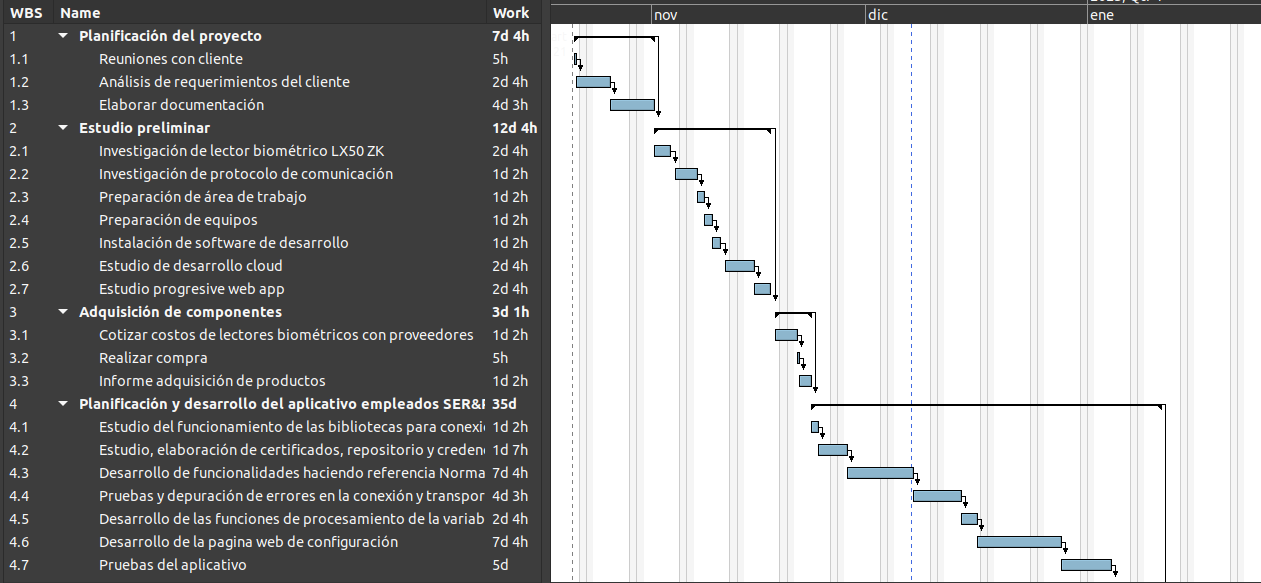
\includegraphics[width=1\textwidth]{./Figuras/ganntParte1.png}
\caption{Diagrama gannt 1/2}
\label{fig:AoN}
\end{figure}

\begin{figure}[htpb]
\centering 
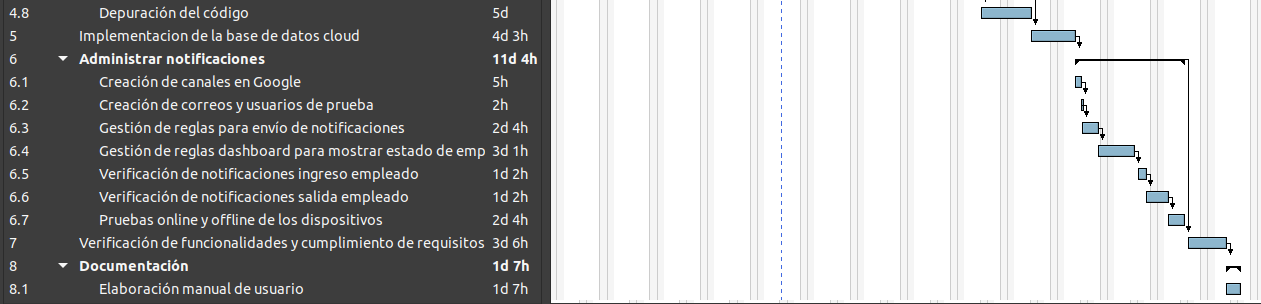
\includegraphics[width=1\textwidth]{./Figuras/ganntParte2.png}
\caption{Diagrama gannt 2/2}
\label{fig:AoN}
\end{figure}


\section{12. Presupuesto detallado del proyecto}
\label{sec:presupuesto}


\begin{table}[htpb]
\centering
\begin{tabularx}{\linewidth}{@{}|X|c|r|r|@{}}
\hline
\rowcolor[HTML]{C0C0C0} 
\multicolumn{4}{|c|}{\cellcolor[HTML]{C0C0C0}COSTOS DIRECTOS} \\ \hline
\rowcolor[HTML]{C0C0C0} 
Descripción &
  \multicolumn{1}{c|}{\cellcolor[HTML]{C0C0C0}Cantidad} &
  \multicolumn{1}{c|}{\cellcolor[HTML]{C0C0C0}Valor unitario} &
  \multicolumn{1}{c|}{\cellcolor[HTML]{C0C0C0}Valor total} \\ \hline
 &
  \multicolumn{1}{c|}{} &
  \multicolumn{1}{c|}{} &
  \multicolumn{1}{c|}{} \\ \hline
 &
  \multicolumn{1}{c|}{} &
  \multicolumn{1}{c|}{} &
  \multicolumn{1}{c|}{} \\ \hline
\multicolumn{1}{|l|}{} &
   &
   &
   \\ \hline
\multicolumn{1}{|l|}{} &
   &
   &
   \\ \hline
\multicolumn{3}{|c|}{SUBTOTAL} &
  \multicolumn{1}{c|}{} \\ \hline
\rowcolor[HTML]{C0C0C0} 
\multicolumn{4}{|c|}{\cellcolor[HTML]{C0C0C0}COSTOS INDIRECTOS} \\ \hline
\rowcolor[HTML]{C0C0C0} 
Descripción &
  \multicolumn{1}{c|}{\cellcolor[HTML]{C0C0C0}Cantidad} &
  \multicolumn{1}{c|}{\cellcolor[HTML]{C0C0C0}Valor unitario} &
  \multicolumn{1}{c|}{\cellcolor[HTML]{C0C0C0}Valor total} \\ \hline
\multicolumn{1}{|l|}{} &
   &
   &
   \\ \hline
\multicolumn{1}{|l|}{} &
   &
   &
   \\ \hline
\multicolumn{1}{|l|}{} &
   &
   &
   \\ \hline
\multicolumn{3}{|c|}{SUBTOTAL} &
  \multicolumn{1}{c|}{} \\ \hline
\rowcolor[HTML]{C0C0C0}
\multicolumn{3}{|c|}{TOTAL} &
   \\ \hline
\end{tabularx}%
\end{table}


\section{13. Gestión de riesgos}
\label{sec:riesgos}

\begin{table}[htpb]
\centering
\begin{tabularx}{\linewidth}{@{}|X|c|c|c|c|c|c|@{}}
\hline
\rowcolor[HTML]{C0C0C0} 
Riesgo & S & O & RPN & S* & O* & RPN* \\ \hline
       &   &   &     &    &    &      \\ \hline
       &   &   &     &    &    &      \\ \hline
       &   &   &     &    &    &      \\ \hline
       &   &   &     &    &    &      \\ \hline
       &   &   &     &    &    &      \\ \hline
\end{tabularx}%
\end{table}




\section{14. Gestión de la calidad}
\label{sec:calidad}



\section{15. Procesos de cierre}    
\label{sec:cierre}

Las actividades de los procesos de cierre estarán a cargo del responsable del proyecto, Ing. Flavio Bolívar Vinueza Barzola.

Se analizará el grado de cumplimiento de la planificación en contraste con su ejecución. Se
detectarán aquellas tareas que no se cumplieron en tiempo y se hará su correspondiente
evaluación a fin de tener esta información en cuenta para otros proyectos. La documentación está en el repositorio Git del proyecto.

Se observará si fue necesario cambiar algún requerimiento durante la ejecución, en tal
caso, se analizarán sus causas y se documentará esta información.

El responsable del proyecto realizará una lista de las técnicas y procedimientos que le
resultaron útiles para cumplir con los objetivos preestablecidos, y las que le hayan generado
retrasos, indicando las posibles causas.

El responsable del proyecto se encargará de agradecer a todas las personas involucradas en el
proyecto. Los gastos del proyecto corren por cuenta del cliente \clientename.

\end{document}
